%  P1 - Geophysical Research Letters version (AGU template agujournal2019.cls). Build: pdflatex, bibtex, pdflatex x2.
%  Draft v0.5 (2026-10-21). Author list, affiliations and ORCIDs to be completed by the authors. AI assistance must be
%  disclosed in the Acknowledgments per AGU policy.
\documentclass[draft]{agujournal2019}
\usepackage{url}
\usepackage{lineno}
% \usepackage[inline]{trackchanges}  % optional (needs soul.sty)
% \usepackage{soul}  % (optional, AGU template)
\usepackage{amsmath,amssymb}
\linenumbers
\draftfalse

\journalname{Geophysical Research Letters}

\begin{document}

\title{Minimum-Seismicity Injection Design Is Convex, and the Value of Design Is Set by Two Numbers}

\authors{[Author 1]\affil{1}, [Author 2]\affil{1}}
\affiliation{1}{[Affiliation to be completed]}
\correspondingauthor{[Name]}{[email]}

\begin{keypoints}
\item Expected induced-event counts under Dieterich seismicity with linear poroelastic coupling are convex in all injection-rate histories
\item Protocol rankings flip with the counting window: step-up schedules can turn from best to worst once post-shut-in events are counted
\item The gain from optimal design follows a theta-curve, confirmed in a pre-registered test at the 2020 Otaniemi stimulation
\end{keypoints}

\begin{abstract}
Studies disagree on which injection protocol minimizes induced seismicity. We prove that, under the Dieterich seismicity-rate model with
Coulomb stress linear in the injection rates, the expected event count over any window is convex in the rate histories of all wells.
Optimal design therefore has a certified global optimum and a unique optimal stress history. A stress-dose invariance makes schedule effects
Jensen gaps controlled by $\Pi=\Delta S_{\max}/A\bar\sigma$, and the value of design also depends on $\theta$, the stress-response time over the
injection time. Protocol rankings reverse with the counting window. At Otaniemi 2018 ($\theta\ll0.1$) the optimum gains 1.6\% over constant
rate. A pre-registered test on the three-times-shorter 2020 stimulation refuted our predicted gain ($\le3$\%; realized 9.1\%) but confirmed
the predicted peak of the gain at $\theta\approx0.1$--1. In a reservoir simulator, two-way fault coupling raised the expected count by 36\% in one test case; with such feedback convexity is no longer guaranteed.
\end{abstract}

\section*{Plain Language Summary}
Pumping water into the ground for geothermal energy or storage can trigger small earthquakes. Operators can change how fast they pump, but
studies disagree on whether it is better to pump steadily, to increase the rate in steps, or to taper off. We show mathematically that, in
the most widely used model of induced earthquake rates, the problem of choosing the pumping schedule has a single best answer that a
computer can find reliably. Part of the disagreement between earlier studies comes from when they stop counting earthquakes: some schedules
look good at the moment pumping stops but cause more earthquakes afterwards. How much a smarter schedule can help depends on two numbers that
can be estimated from data. We tested this on two stimulations of a 6-km-deep geothermal well in Finland. In 2018 the best schedule would
have helped little; in 2020, when pumping was three times shorter, it would have helped about six times more, as the theory's curve predicts,
though more than our own advance forecast.

\section{Introduction}
Rate control is the main operational lever against injection-induced seismicity
\cite<e.g.,>{Zang2018,Kwiatek2019}. Synthetic and laboratory studies reach opposite conclusions: constant-rate injection is best in some
\cite{Boyet2024}, step-up schedules in others \cite{AlghannamJuanes2020}, and optimal-control formulations have been proposed for specific
models \cite{Candela2022,Hill2024,GutierrezStefanou2024,GutierrezStefanou2026,Walter2026}; for Otaniemi, \citeA{Kim2025} combine a robust tracking controller with a scenario search and find stimulations that outperform the 2018 schedule. What is missing is a statement of the structure of the design problem itself --- whether its
optimum is global, what the optimum looks like, and when the schedule matters at all. We provide this for the Dieterich (1994) framework
with linear poroelastic coupling and test the resulting predictions on field data, including one pre-registered test whose quantitative
prediction failed.

\section{Theory}
\subsection{Seismicity Model}
For a fault patch with effective normal stress $\bar\sigma$, direct-effect parameter $A$ and background stressing rate $\dot\tau_r$, the
Dieterich rate $R$ satisfies $\mathrm{d}\gamma/\mathrm{d}t=(1-\gamma\dot S)/a$, $R=r/(\gamma\dot\tau_r)$, with $a=A\bar\sigma$ and
$t_a=a/\dot\tau_r$ \cite{Dieterich1994,HeimissonSegall2018}. For any Coulomb stress history $S(t)=\dot\tau_r t+\Delta S(t)$,
\begin{equation}
\frac{N(T)}{r}=t_a\ln\!\left(1+\frac{1}{t_a}\int_0^T e^{S(s)/a}\,\mathrm{d}s\right),\qquad
\Delta S(x,t)=\sum_w\int_0^t g_w(x,t-s)\,q_w(s)\,\mathrm{d}s ,
\label{eq:N}
\end{equation}
where $g_w$ is the Coulomb stress response at $x$ to a unit rate step at well $w$ (linear poroelasticity, any heterogeneity).

\subsection{Convexity}
\textbf{Theorem 1.} \emph{With $\Delta S$ linear in the rates $q$, the expected excess count $E(T;q)=N/r-T$ is convex in $q$ for every $T$
and patch; positive sums over patches are convex. With linear constraints (volume, rate bounds, linear pressure caps), minimum-seismicity
design is a convex programme.}

\emph{Proof.} Write $N/r=t_a\ln\int e^{h_s(q)}\mathrm{d}\mu(s)$ with the measure $\mu=\delta_*+t_a^{-1}\mathrm{d}s$ on
$\{*\}\cup[0,T]$, $h_*=0$ and $h_s(q)=(\dot\tau_r s+\Delta S(x,s;q))/a$, affine in $q$. Hölder's inequality with exponents $1/\lambda$ and
$1/(1-\lambda)$ gives $\int e^{\lambda h(q_1)+(1-\lambda)h(q_2)}\mathrm{d}\mu\le(\int e^{h(q_1)}\mathrm{d}\mu)^\lambda(\int e^{h(q_2)}\mathrm{d}\mu)^{1-\lambda}$;
taking logarithms proves convexity. $\square$

Because the atom fixes $h_*=0$, equality in Hölder forces $h(q_1)=h(q_2)$ $\mu$-a.e.: the optimal \emph{stress history} is unique, while
the rate history is unique only if the response operator is injective (diffusion filters high frequencies, so many schedules share the
optimal stress). The KKT conditions equalize the marginal events per unit volume where the rate bounds are inactive, which produces
bang--singular--bang optima. If $\int_0^\infty g\,\mathrm{d}t=S_{ss}$ is finite, Fubini gives $\int_0^\infty\Delta S\,\mathrm{d}t=VS_{ss}$
for every schedule of volume $V$ (stress-dose invariance); for $T\ll t_a$, $E\approx\int(e^{\Delta S/a}-1)\mathrm{d}t$ and Jensen's
inequality makes schedule effects gaps that scale with the variance of $\Delta S/a$, i.e., with $\Pi=\Delta S_{\max}/a$. Peak-rate
minimization is a linear programme, and the count--peak Pareto front is convex.

\subsection{The $\theta$-law}
For one first-order kernel $\theta\dot s=u-s$ (time in units of the injection time) the optimum is a maximum-rate charging arc, a
constant-stress plateau (singular arc) and a maximum-rate burst before shut-in. Its gain over constant rate, $G(\Pi,\theta,u_{\max})$, is
known in closed form (Supporting Information Text S1), vanishes for $\theta\to0$ (the stress follows the rate) and $\theta\to\infty$ (the
stress integrates the volume) and peaks at $\theta\approx0.1$--1. Before field data are fitted, $\Pi$ and $\theta$ indicate whether design
can pay.

\section{Synthetic Test: The Counting-Window Artefact}
In a 3-D diffusion test (Figure~1; parameters in Text S2) the four-step step-up schedule gives 25\% fewer excess events than constant rate
when counting stops at shut-in, but 4\% \emph{more} when the post-injection tail is counted; the taper is worse in both windows; the global
optimum gives $-13.5$\% and $-4.7$\%, the lowest total of all admissible schedules. In 26\% of randomly sampled sites step-up flips from best
to worse once post-shut-in events are counted. Convexity was checked by 2000 random midpoint tests (no violation; Figure~S1) and multistart
optima agreed to solver tolerance. Protocol comparisons must therefore state the counting window.

\section{Field Tests at Otaniemi}
We used public pumping data \cite{Kukkonen2023} and catalogues \cite{Leonhardt2021,Kwiatek2022data} of the 2018 (OTN-3) and 2020 (OTN-2)
stimulations of the Otaniemi geothermal project \cite{Kwiatek2019,Kwiatek2022}. A linear multi-exponential kernel maps rate to wellhead
pressure, the Dieterich model with a pressure threshold $P^*$ maps pressure to event rate, and expected counts of the actual, the
constant-rate and the optimal schedule (same volume, same rate bounds) are compared. Every test, prediction and verdict rule was fixed before
the data were examined (Text S3).

\textbf{2018} (18,433~m$^3$ in 49~d, 23,854 events above $M_c=-0.95$; Figure~3). The fit is excellent in-sample (correlation 0.998), the
post-injection tail is over-predicted by 50\%. Expected counts: 23,828 (actual), 21,546 (constant), 21,211 (optimum), $\Pi=3.06$: the
optimum gains only 1.6\%, an order of magnitude less than the $\Pi$-law estimate (13\%), while the irregular operator schedule costs 11\%.
The fitted stress-carrying modes have $\theta\ll0.1$, where the $\theta$-scan predicts small gains and large penalties for irregularity.

\textbf{2020, pre-registered} (2,884~m$^3$ in 16.1~d, 2,846 events above $M_c=-1.45$; Figure~2). The Dieterich fit passed (correlation
0.998, tail +8\%) and the 2018 parameters transfer to 2020 (correlation 0.985). We predicted a gain $\le3$\% assuming $\theta\ll0.1$ as in
2018. \textbf{This prediction was refuted:} 2,834 (actual), 2,286 (constant), 2,078 (optimum) events, a gain of 9.1\%, and +24\% for the
operator schedule. The pre-registered $\theta$-scan prediction was \textbf{confirmed}: the gain peaks at $\theta=0.26$ (14.0\%) inside the
predicted interval [0.05,~1] (Figure~2c). The prediction failed because its input was wrong: the 2020 injection was three times shorter, so
the same crustal response times give $\theta\approx0.26$--0.77 for 73\% of the kernel's steady-state pressure. A post-hoc forecast that
weights the 2018 $\theta$-curve by the 2020 kernel shares gives 6.5\% (realized 9.1\%; $\Pi$-law 15.6\%). We report this as consistent, not
as confirmation. With the operator's eight pauses imposed, the optimum is only 3.1\% better than the actual schedule, and a design made
from a degenerate calibration ($P^*$ at its bound) performed 2.9 times worse than constant rate: design requires an identifiable threshold.

The theory applies to shear reactivation by pore-pressure diffusion, not to tensile-growth emissions: at the \"Asp\"o hard-rock laboratory,
hydraulic-fracturing acoustic emissions follow hydraulic energy rather than the Dieterich response to pressure (companion reanalysis, in preparation).

\section{Inside a Reservoir Simulator}
Within a simulator report step the Coulomb stress of a fault face changes linearly, so the Dieterich state has the exact update
$\gamma(t+h)=(\gamma-1/\dot S)e^{-\dot Sh/a}+1/\dot S$. We implemented this per fault face in the open reservoir simulator ResSim together
with a stochastic catalogue and optional two-way coupling, in which reactivated faces ($\mathrm{CFF}\ge0$) conduct (Figure~4). Resolved
stresses match a hand calculation to $10^{-3}$~bar and the in-run count matches the closed form for constant stressing (1.32734 vs
1.32734 events). In an injector--fault case, two-way coupling turns the sealing fault into a conduit (cross-fault pressure jump 43.7 to
$\approx5$~bar) and raises the expected count from 352 to 479 events (+36\%) relative to one-way monitoring. Because transmissibility then
depends on $q$, Theorem~1 no longer applies. In a companion simulation study (in preparation) the count stays convex for passive faults
but loses convexity once the reached fault-transmissibility multiplier exceeds about 1.7--2.4; re-linearizing around the current design
(re-simulation plus a convex offset correction, as supported by the simulator) is then a local method without a global certificate.

\section{Discussion and Conclusions}
Minimum-seismicity design under Dieterich seismicity with linear coupling is convex: its optimum is global and cheap, the optimal stress
history is unique, and peak-rate design is a linear programme. Protocol disagreements in the literature are partly a counting-window
artefact. Whether design pays is set by $\Pi$ and $\theta$: at fast-responding sites ($\theta\ll0.1$) the schedule should be smooth but
optimization gains little; near $\theta\approx0.1$--1 gains approach 10--15\%. The two Otaniemi stimulations --- same reservoir, different
injection durations --- move along this curve as predicted, although our pre-registered point forecast for 2020 was too low. Limitations:
stationary Dieterich populations without triggering (ETAS breaks convexity), constant $\bar\sigma$, expected rather than realized counts,
and a $\theta$-law supported post hoc at a second stimulation of the same reservoir; an independent site with a public hourly injection
log is the next test.

\section*{Open Research}
Data: Otaniemi 2018 catalogue \cite{Leonhardt2021}, Otaniemi 2020 catalogue \cite{Kwiatek2022data}, Otaniemi hydraulics
\cite{Kukkonen2023}, all CC BY 4.0. Code: experiment scripts, figure data and the ResSim simulator (fault
mechanics in \texttt{faultmech.cpp}, figure rendering in \texttt{figure.cpp}) will be archived on Zenodo [DOI to be added at
submission]; pre-registrations and the findings log are included.

\acknowledgments
[Funding.] Parts of the analysis code and text were drafted with AI assistance and verified by the authors [adapt to AGU policy].

\bibliography{refs}

\clearpage
\begin{figure}
\centering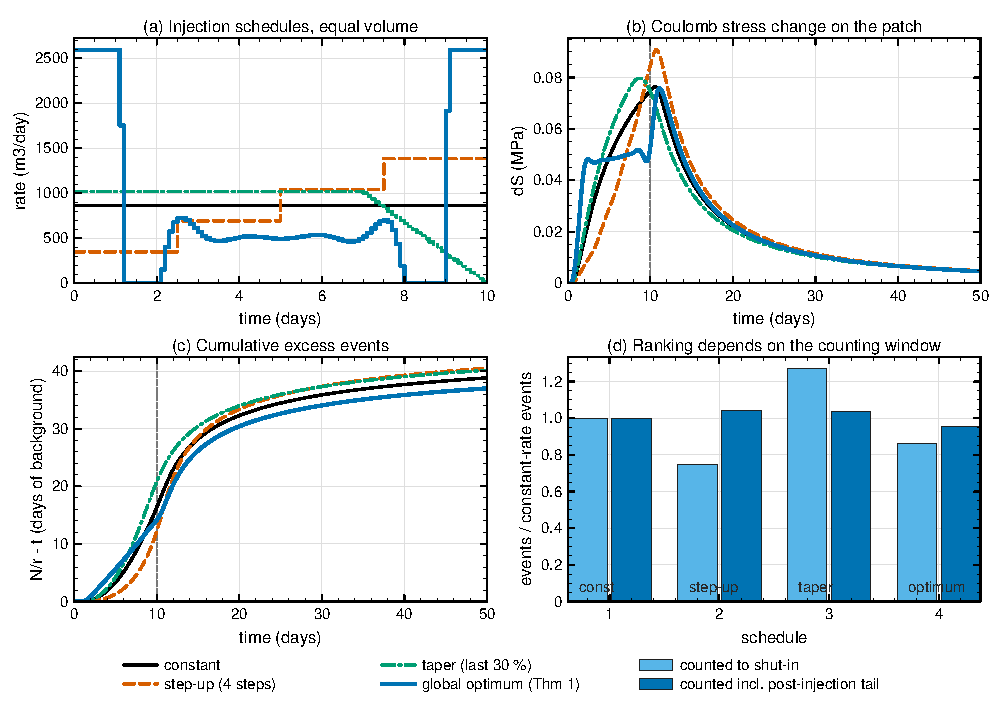
\includegraphics[width=\textwidth]{figs/Figure1.pdf}
\caption{Synthetic test. (a) Equal-volume schedules; the optimum has the bang--singular--bang structure. (b) Coulomb stress on the patch.
(c) Cumulative excess events; dashed: shut-in. (d) Events relative to constant rate when counting stops at shut-in (light) and with the
post-injection tail (dark): 1 constant, 2 step-up, 3 taper, 4 global optimum.}
\end{figure}
\begin{figure}
\centering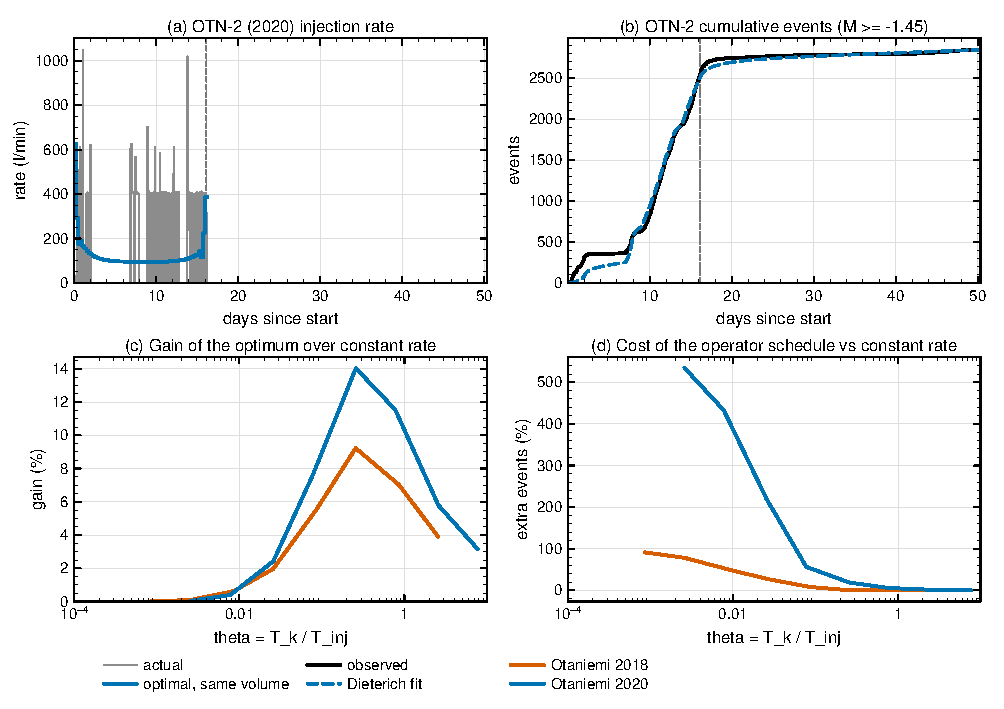
\includegraphics[width=\textwidth]{figs/Figure2.pdf}
\caption{Otaniemi 2020 (OTN-2) and the $\theta$-law at two stimulations. (a) Injection rate and the optimal schedule with the same volume.
(b) Cumulative events and Dieterich fit. (c) Gain of the global optimum over constant rate versus $\theta=T_k/T_{inj}$ (kernel time rescaled).
(d) Extra events of the operator schedule relative to constant rate.}
\end{figure}
\begin{figure}
\centering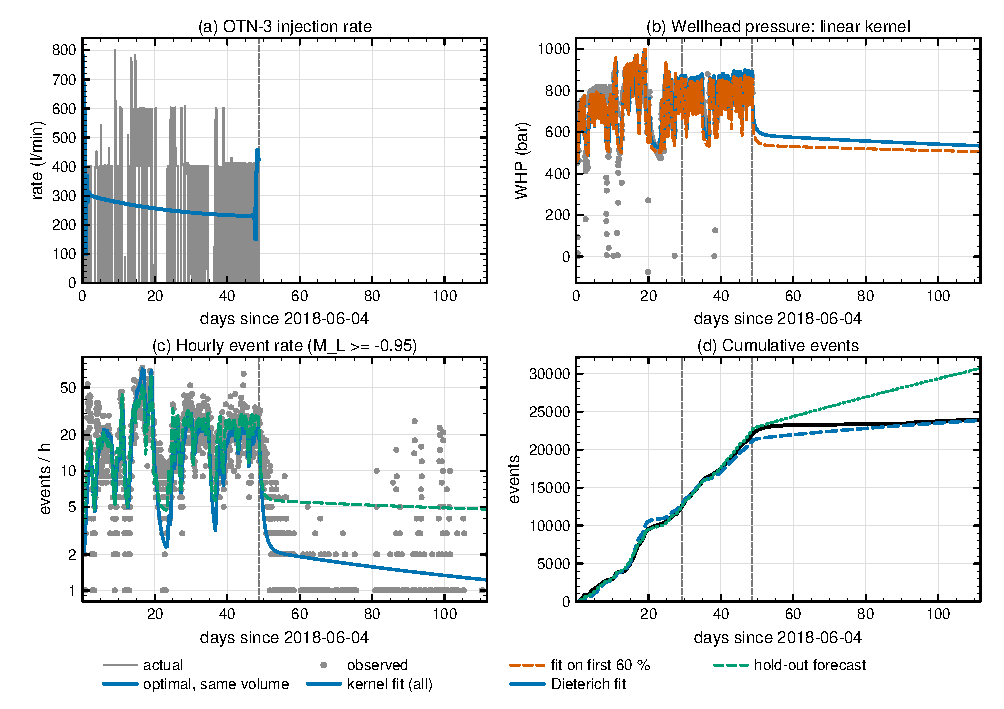
\includegraphics[width=\textwidth]{figs/Figure3.pdf}
\caption{Otaniemi 2018 (OTN-3). (a) Injection rate and optimal schedule. (b) Wellhead pressure and the linear kernel (all data and first
60\%). (c) Hourly event rate, Dieterich fit and hold-out forecast. (d) Cumulative events. Vertical lines: end of training window, shut-in.}
\end{figure}
\begin{figure}
\centering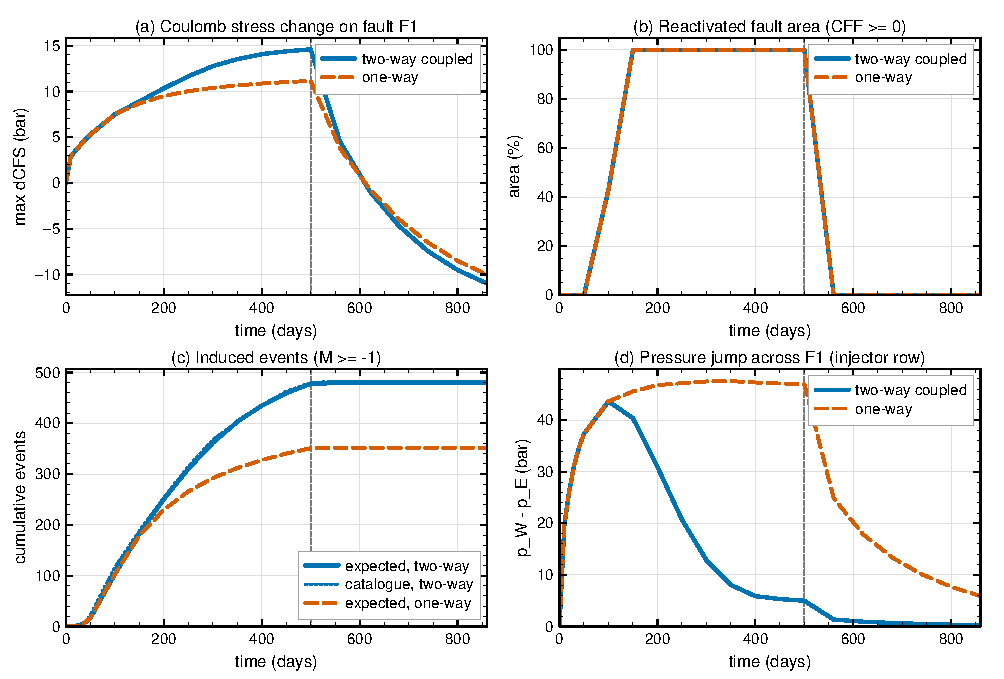
\includegraphics[width=\textwidth]{figs/Figure4.pdf}
\caption{Fault mechanics inside the reservoir simulator, two-way coupling (reactivated faces conduct) versus one-way monitoring.
(a) Maximum Coulomb stress change on the fault. (b) Reactivated fault area. (c) Expected and sampled events. (d) Pressure jump across the
fault in the injector row. Dashed: shut-in.}
\end{figure}

\end{document}
